\section{Introduction}
\label{introduction}

\subsection{How to read this manual}
\label{howtoread}
This manual will guide you through the execution of the steps that will bring you to know and use the features of Romeo, at best. The document is divided in four principal sections:
\begin{itemize}
\item \textbf{Getting started:} which will provide you the instructions to install and uninstall the software. It also gives you an overview of the main window of Romeo;
\item \textbf{Set up analysis:} which will guide you through the execution of the necessary steps, that allow you to perform an analysis;
\item \textbf{Execution of an analysis:} which will provide you the instructions to manage and execute an analysis;
\item \textbf{Visualization and exportation of results:} which will guide you through the management of the results obtained from the analysis.
\end{itemize}
The \textbf{Glossary} appendix contains definitions of the terms that needs an explanation, for reasons of clarity. These terms are marked in the manual with a subscript \lq\lq{}G\rq\rq{} in bold.

\subsection{Overview}
\label{overview}
Romeo is an open source tool that can provide the application of cluster analysis to biomedical data. Furthermore, it is possible to extract some features\g{} of interest from the images and combine them before performing clustering.\\
This technique is used to automate and facilitate the delineation of anatomical structures and other regions of interest, in medical images. The procedure, can accelerate the processing speed and accuracy of the diagnosis, allowing to locate pathological 	tissues and measure tissue volumes. It has thus great potential for
prevention, prognosis, and treatment.\\
Below, a schematic representation of the pipeline of analysis of a cluster analysis applied to biomedical image (fig. \ref{pipeline}).
\begin{figure}[!h]
\centering
	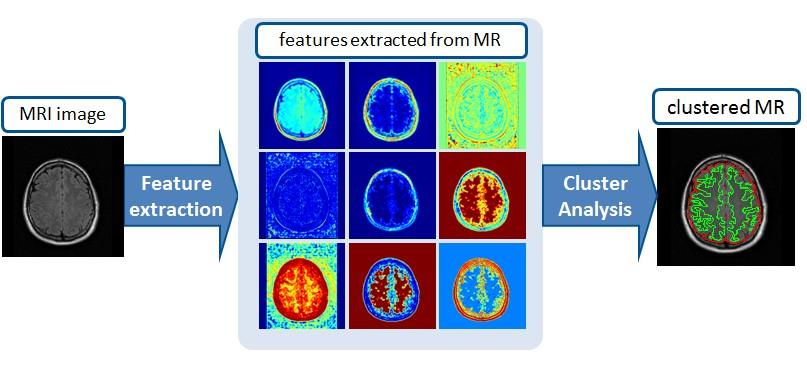
\includegraphics[scale=0.5]{./Images/pipe}
	\caption{\textit{Feature extraction and Cluster Analysis of a MR image}}
	\label{pipeline}
\end{figure}

\subsection{Why Romeo?}
\label{whyromeo}
\begin{itemize}
\item \textbf{Intuitive User Interface\\} Romeo has an intuitive Grafic User Interface that allows it to be used by expert and not expert ICT users;
\item \textbf{Various cluster algorithms\\} Romeo is the only stand-alone software that integrates three types of Cluster Algorithms by default. In fact, it implements: \textbf{K-means}, \textbf{Fuzzy C means} and \textbf{Hierarchical} algorithms;
\item \textbf{Supports major data formats\\} This tool can work with 2D, 3D, 2D-t and 3D-t images and supports these file formats: \verb!.PNG!, \verb!.JPG!, \verb!.BPM!, \verb!.AVI!, \verb!NIfTI! and \verb!Analyze 7.5! ;
\item \textbf{Various feature extractors\\} Romeo implements fifteen different Feature Extractors;
\item \textbf{Independence from file-system\\} Once Romeo has imported data, the user has the freedom to change the location of the imported images in its file-system. In fact, the software saves the images inside itself. Once the user wants to export some image results, Romeo asks the path where the files have to be saved.
\end{itemize}

\subsection{Romeo Features}
\label{features}
\begin{itemize}
\item \textbf{Apply mask\\} Enables users to import a mask and associate it to another image. That mask, works like a filter of interest on the imported image; in other words, it delimits the region which will be analyzed;
\item \textbf{Create groups of Subjects\\} Enables users to create customized sets of Subjects\g{} (an image plus its mask), allowing to perform the algorithms on different images simultaneously;
\item \textbf{Create Protocols\\} Enable users to create customized Protocols\g{} (a set of Feature Extractors plus one o none cluster algorithm\g{}). Each algorithm can be customized with its own parameters (like window size, GLCM etc\dots{});
\item \textbf{Create Dataset\\} Enables users to create a customized analysis, formed by a group of Subjects\g{} and one or more Protocols\g{}. The Dataset\g{} also memorize the results of the analysis and permits the user to export them;
\item \textbf{Possibility of extension with other algorithms\\} Enables developers to extend the set of feature extractors and cluster algorithms with new ones, compatible with supported format files. 
\end{itemize}